

% This is mymiccaipaper.tex the demonstration file of
% MICCAI 2006 for Latex2e
% adapted from LLNCS.DEM from
% the LaTeX macro package from Springer-Verlag
% for Lecture Notes in Computer Science,
% version 2.2 for LaTeX2e
%
%\documentclass[runningheads]{llncs}
\documentclass[a4paper, lmargin=1.925cm, rmargin=1.925cm,tmargin=2.54cm,bmargin=4.94cm]{spie}
%
\usepackage{makeidx}  % allows for indexgeneration
%st added this to help with anonymisation
%otherwise it took my name from one of the eps file
%This still got overwritten by the last eps file,
%had to manually pull the author out of that.
\pdfinfo{
%letterpaper,
%colorlinks,
%urlcolor=black,
pdfpagemode=none,
pdftitle={blank},
pdfauthor={anonymous},
pdfcreator={},
pdfsubject={},
pdfkeywords={}
}
		  
%
\usepackage{multirow}
\usepackage{graphicx}
\usepackage{rotating}
\usepackage{array}
\usepackage{pifont}
\graphicspath{{pics/}{figs/}}
% list here all the paths to your figure folders
\usepackage{glossaries} %st - put this in to deal with acronyms tidily
%\usepackage[acronym=true,description]{glossaries} %st - put this in to deal with acronyms tidily
\newacronym[description=root mean square]{RMS}{RMS}{root mean square}
\newacronym[description=iterative closest point]{ICP}{ICP}{iterative closest point}
\newacronym[description=computed tomography]{CT}{CT}{computed tomography}
\newacronym[description=point cloud library]{PCL}{PCL}{point cloud library}
\newacronym[description=simultaneous localisation and mapping]{SLAM}{SLAM}{simultaneous localisation and mapping}
\newacronym[description=graphics processing unit]{GPU}{GPU}{graphics processing unit}
\newacronym[description=fiducial registration error]{FRE}{FRE}{fiducial registration error}
\newacronym[description=fiducial localisation error]{FLE}{FLE}{fiducial localisation error}
\newacronym[description=target registration error]{TRE}{TRE}{target registration error}
 %removed relative path and replaced with symbolic link in this directory, see makefile.

\begin{document}
%
%\frontmatter          % for the preliminaries
%
%\authorrunning{S. Thompson et al.}   % abbreviated author list (for running head)
%\pagestyle{headings}  % switches on printing of running heads
%\pagestyle{empty}  % switches off printing of running heads
%
%\mainmatter              % start of your contributions
%
\title{Are fiducial registration error and target registration error correlated? Using SciKit-SurgeryFRED for teaching and user interface research.}
%\titlerunning{Laproscope Calibration}  % abbreviated title (for running head)
%
%\author{Stephen Thompson \and Matt Clarkson \and Johanned Totz \and Yi Song \and Danail Stoyanov \and David Hawkes }
%
\author{Stephen~Thompson\supit{1}, Tom~Dowrick\supit{1}, Mian~Ahmad\supit{1}, Matthew~J.~Clarkson\supit{1}
\skiplinehalf
\supit{1}Wellcome/EPSRC Centre for Interventional and Surgical Science, University College London, United Kingdom \\
}

%
%
%%%% modified list of authors for the TOC (add the affiliations)
%\tocauthor{Stephen Thompson (University College London),
%Matt Clarkson (University College London),
%Johannes Totz (University College London),
%Yi Song (University College London),
%David Hawkes (University College London)
%}
%
%\institute{Centre for Medical Image Computing, University College London.
%}

% The following lines are used to remove authors and affiliations from
% the front page and running titles
%\author{-, -, -}
%\authorrunning{-}
%\tocauthor{-}
%\institute{-}

\maketitle              % typeset the title of the contribution

%\begin{abstract}
%Understanding the relationship between fiducial registration error (FRE) and target registration error (TRE) is important for the correct use of interventional guidance systems. Whilst it is well established that TRE is statistically independent of FRE, system users still struggle against the intuitive assumption that a low FRE indicates a low TRE. We present the SciKit-Surgery Fiducial Registration Educational Demonstrator and describe its use. SciKit-SurgeryFRED was developed to enable remote teaching of key concepts in image registration. SciKit-SurgeryFRED also supports research into user interface design for image registration systems. 

SciKit-SurgeryFRED can be used to enable remote tutorials covering the statistics relevant to image guided interventions. Students are able to place fiducial markers on pre and intra-operative images and observe the effects of changes in marker geometry, marker count, and fiducial localisation error on TRE and FRE. SciKit-SurgeryFRED also calculates statistical measures for the expected values of TRE and FRE. Because many registrations can be performed quickly the students can then explore potential correlations between the different statistics. 

SciKit-SurgeryFRED also implements a registration based game, where participants are rewarded for complete treatment of a clinical target, whilst minimising the treatment margin. We used this game to perform a remote study on registration and simulated ablation, measuring how user performance changes depending on what error statistics are made available. The results support the assumption that knowing the exact value of target registration error leads to better treatment. Display of other statistics did not have a significant impact on the treatment performance.  

%\end{abstract}

\section{Introduction}
The fact that \gls{FRE} is uncorrelated with \gls{TRE} is well established 
\cite{fitzpatrick2009}. In spite of this, many students and users of clinical guidance systems struggle to 
correctly interpret \gls{FRE} and residual errors in general. 
SciKit-SurgeryFRED (Fiducial Registration Educational Demonstrator)
 \cite{stephen_thompson_2020_3946090} was developed using the 
SciKit-Surgery \cite{PMID:32436132} libraries to probe the causes of misconceptions 
about \gls{FRE} and \gls{TRE}. SciKit-SurgeryFRED was developed specifically to support on line learning during the enforced lockdowns of 2020, but also provides tools to enable research into user interface design for image guidance systems. SciKit-SurgeryFRED is open 
source software and we encourage researchers and educators to use and contribute to it. 

In this paper we introduce the SciKit-SurgeryFRED application and show how it
be used as an educational tool and as a more general purpose library for
simulation of registration for image guided interventions.

The tutorial utilises questioning strategies within the application, analysis, synthesis and evaluation levels of Bloom's taxonomy \cite{blooms_tax}.

If we change the error model to something non normal would we get correlation between FLE and TRE? Should try this and include.

Include something on non-isotropic errors.

Include something on systematic errors


\section{Methods}
SciKit-SurgeryFRED implements a simple user interface, Figure \ref{fig:surgery_fred}, to demonstrate registration of a pre-operative image to intra-operative space. At startup a target is placed at a random location within the pre-operative image, shown as a red circle. The standard deviation of the \gls{FLE} is randomly sampled from a uniform distribution 
between 0.5 and 5.0 pixels \footnote{All units are in pixels, as the concepts being explored do not depend on the units used. Figure \ref{fig:surgery_fred} shows a brain MRI 458x512 pixels, by design SciKit-SurgeryFRED should work with other images of arbitrary dimensions.}. By default the \gls{FLE} is modelled as an isotropic (in 3 dimensions), normally distributed, and independent random variable, though this can be easily changed. The variance of the \gls{FLE} is shown at the top left (as expected value), along with number of number of fiducial markers. 

\begin{figure}
	\begin{center}
	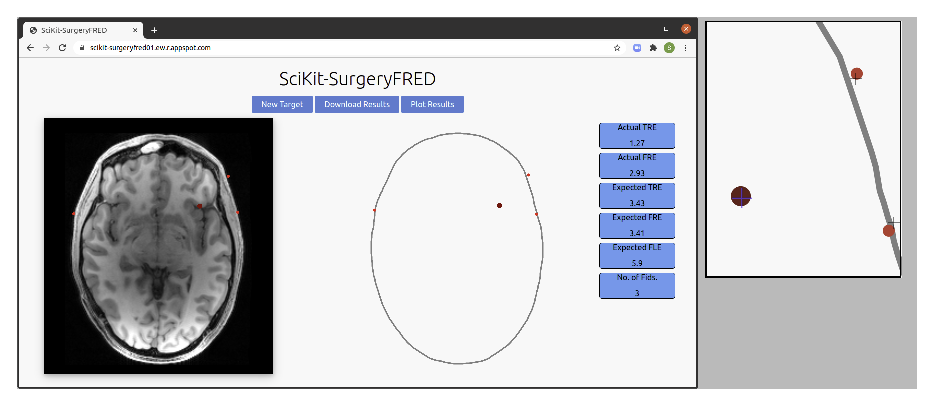
\includegraphics[width=0.9\linewidth]{scikit-surgeryfred_gui.eps}
		\caption{\label{fig:surgery_fred}SciKit-SurgeryFRED graphical user interface after 3 fiducial markers placed. The red sphere in the pre-operative image (left) represents a clinical target, which is located in the
		intra-operative space (middle) by fiducial based registration, using the fiducial markers (green). FLE is added to each marker in the intra-operative image, this is more clearly visible on the zoomed in images at the right. The resulting registration results in a TRE, shown by the misalignment of the red circle and crosshair 
		on the enlarged image at right. TRE and other statistics are shown across the top
		of the window.}
	\end{center}
\end{figure}

Clicking either image adds a fiducial marker to both images. The marker is added to the pre-operative image with no \gls{FLE}. \gls{FLE} is added to the marker location in the intra-operative image, visualised as the misalignment between the green circle centre and the cross-hair. Once sufficient markers are placed ($>2$) the two sets of markers are registered as per \cite{Arun1987}. The expected values (variance) of the \gls{FRE} and \gls{TRE} are calculated 
as per \cite{Fitzpatrick1998}. The registration and statistical algorithms are implemented in SciKit-SurgeryCore \cite{matt_clarkson_2020_3965731}. The student can use this interface together with the
online tutorial 
to explore the relationships between the various statistics and error measures. During use the registration results are 
written to a log file, which can then be used to explore correlation between the different data, an example plot is shown in Figure \ref{fig:correlation}. 
The student should be able to see first hand that, as expected, \gls{FRE} is uncorrelated with \gls{TRE}.

\begin{figure}
	\begin{center}
	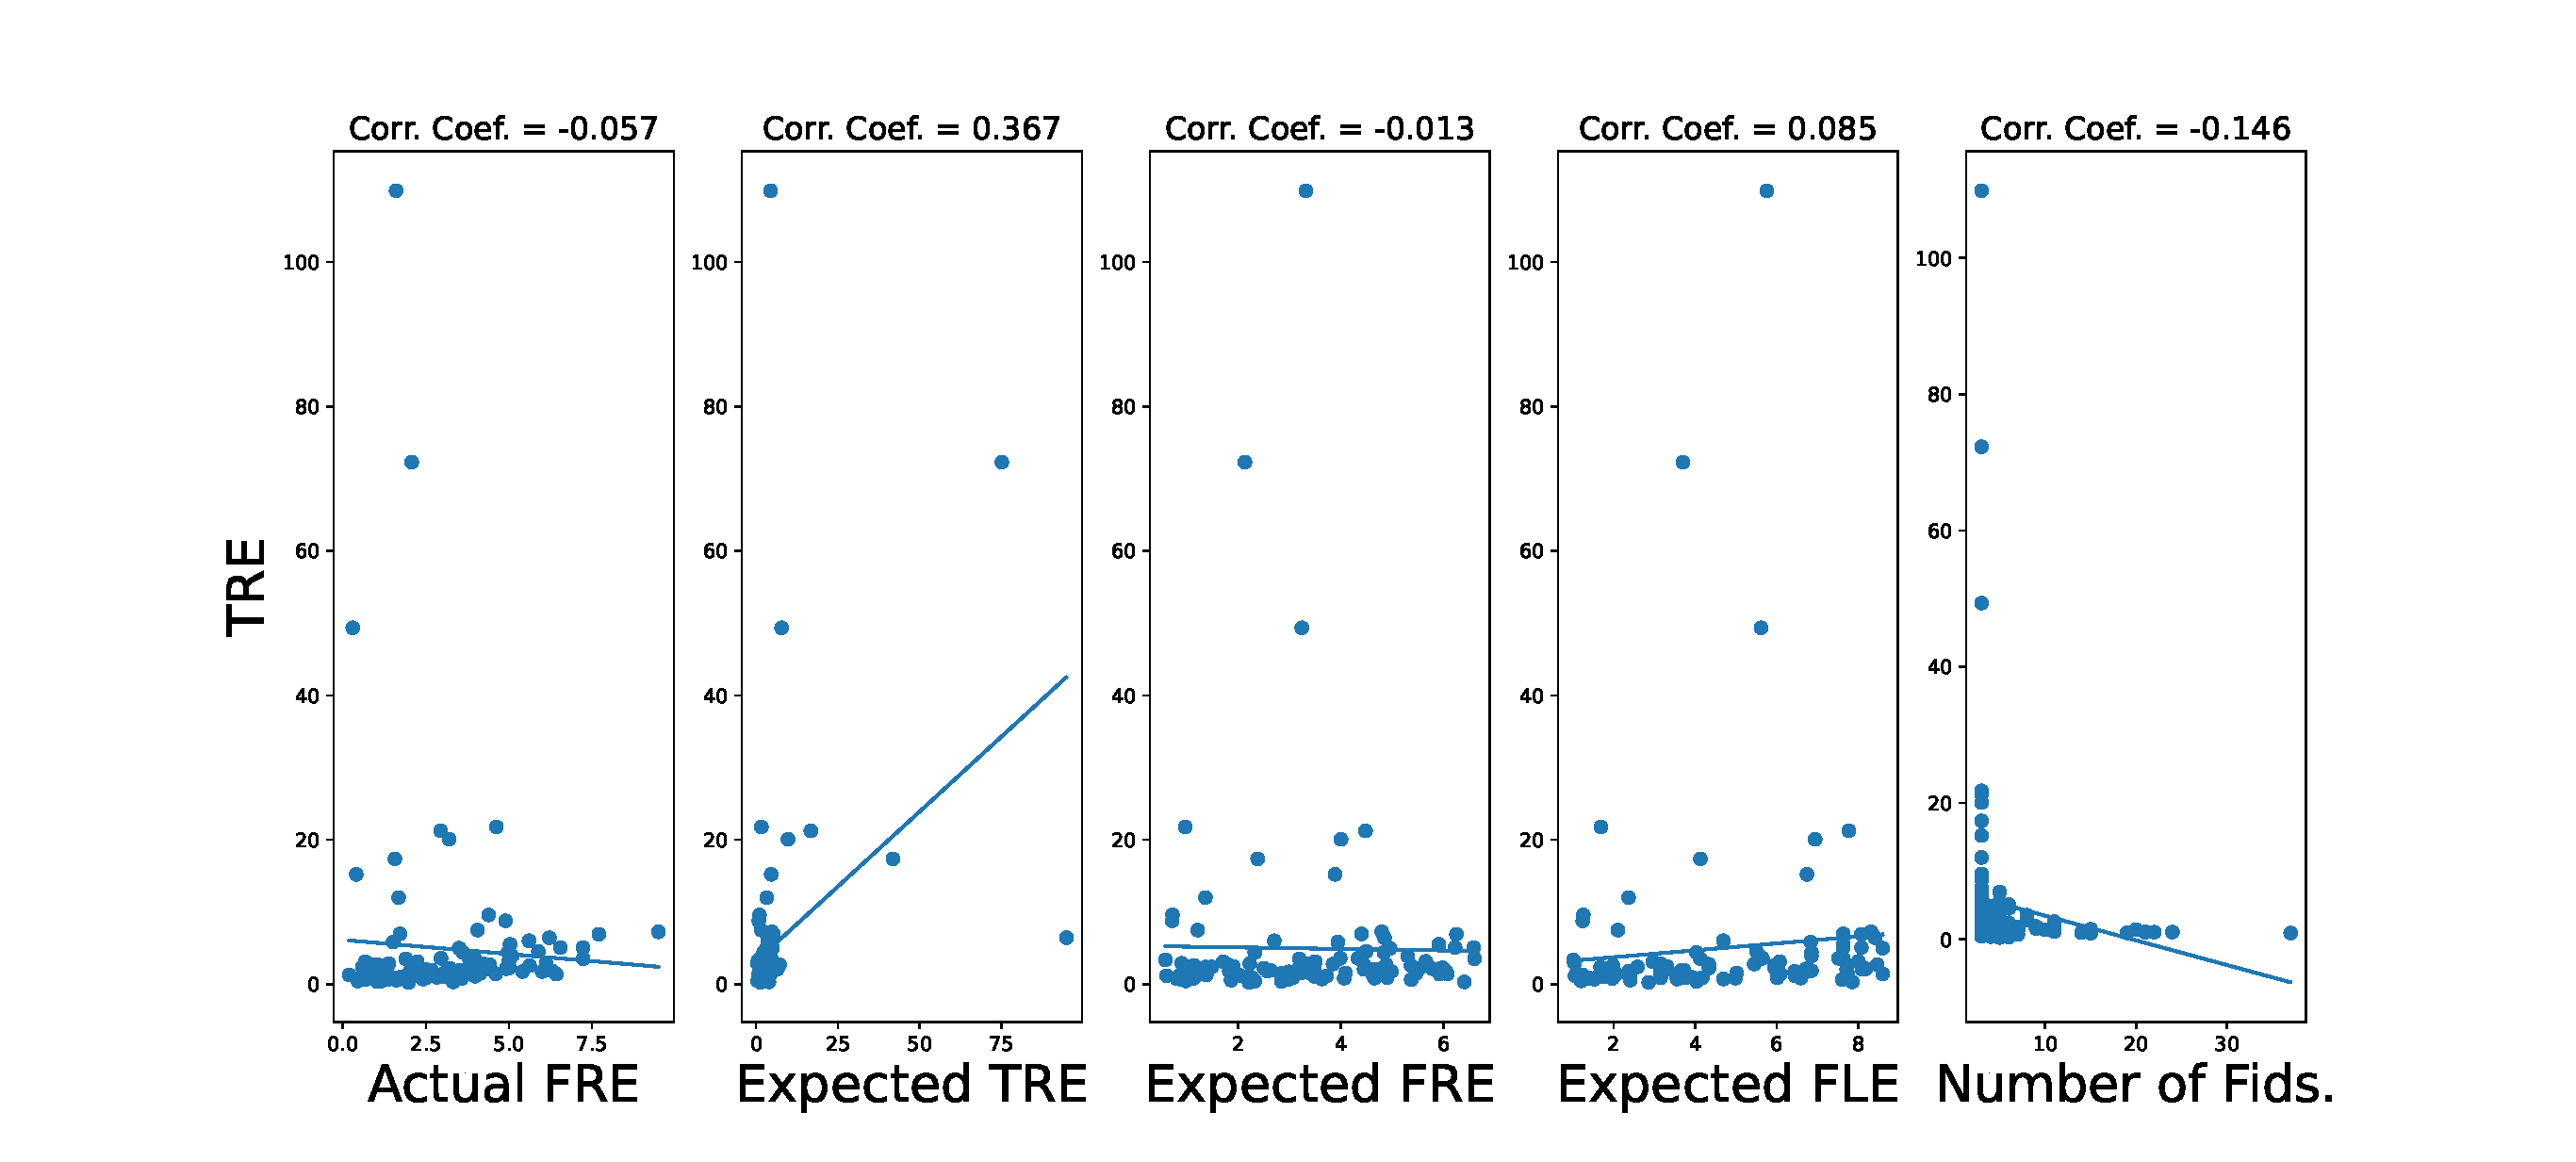
\includegraphics[width=0.9\linewidth]{SciKit-SurgeryF.R.E.D._Correlation_Plots.eps}
		\caption{\label{fig:correlation}Plots of TRE against various error measures, generated by 
		120 user registrations.}
	\end{center}
\end{figure}

\subsection{Game Based Usability Study}
Once the students have an understanding of what statistics can be used to estimate \gls{TRE}, we wanted to test 
how knowledge of a particular statistic affects optimal treatment planning. We designed a serious game to 
do this. After registration the students are able to set a treatment margin and ablate the target. The goal is 
to treat 100\% of the target with minimal ablation of surrounding tissue. A score of 1000 was awarded for complete ablation and 0 
for anything less. From this 10 times the percentage volume of any surrounding tissues ablated is subtracted. So 
treatments failing to treat 100\% of the target will receive a negative score. 
Successful treatments will score between 0 and 1000, depending on the margin size. The optimum treatment 
margin is the actual \gls{TRE} for a given registration.

Each student participated in the game, performing 20 simulated ablations. For the first four ablations they were told the 
actual \gls{TRE}. After that they performed 16 more ablations and were shown one of four randomly selected statistics on which to base their decision,
the expected values of the TRE/FRE, the actual FRE, the expected value of the FLE. Scores were recorded.


\section{Results}
\subsection{\fred as a Teaching Aid}

\fred (v0.0.3)\cite{stephen_thompson_2020_3946090} was used at our Medical Summer School in 2020 with a cohort of 5 students. Informal feedback indicated that it had improved their
understanding
of fiducial based registration. \fred also forms part of the \gls{BARD} which 
was a finalist at the MICCAI 2020 educational challenge 
\footnote{\href{https://miccai-sb.github.io/materials.html}{https://miccai-sb.github.io/materials.html}}. 

\subsection{Extension to Anisotropic Errors}
We simulated an anisotropic independent \gls{FLE}, with \gls{FLE} in the x 
direction being 3 times that in the y and z, as described in Section \ref{sec:anis_method}.
Errors were scaled so that the 
expected absolute value of the \gls{FLE} was the same as for the isotropic case. 
\fred was then used to perform at least 200 simulated registrations, the results of
which are shown in Fig. \ref{fig:anis_error}. 

\begin{figure}
	\begin{center}
			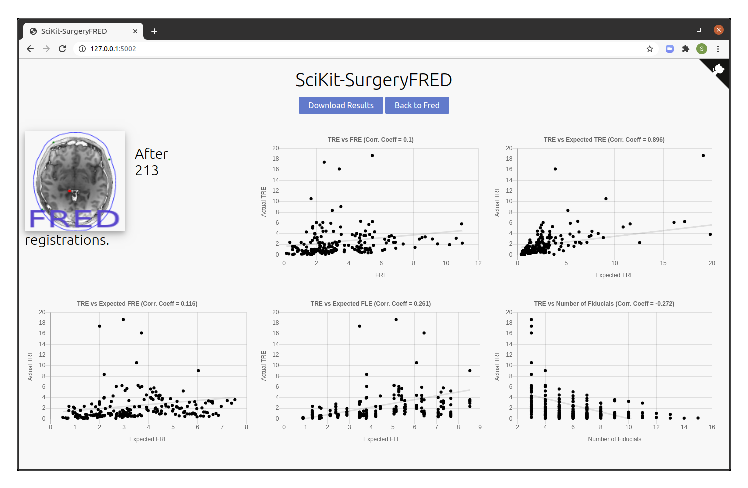
\includegraphics[width=0.9\linewidth]{images/anisitropic_error.eps}
		\caption{\label{fig:anis_error}Results of over 200 registrations using an anisotropic model of {FLE}}
	\end{center}
\end{figure}

It was apparent when performing the registrations that the majority of target 
registration error was in the x direction. However this is not communicated in the 
statistics of Figure \ref{fig:anis_error}. It would be an interesting extension 
exercise to use \fred to explore ways of communicating anisotropic errors during 
treatment.

\subsection{Addition of Systematic Errors}
We added a systematic \gls{FLE} as an isotropic uniform random variable, in the range
-0.5 to 0.5, as described in Section \ref{sec:sys_method}. This error will be applied to all fiducial markers for a 
given registration. We performed at least 200 simulated registrations using \fred, the results of which are shown in Fig. \ref{fig:sys_error}.
\begin{figure}
	\begin{center}
			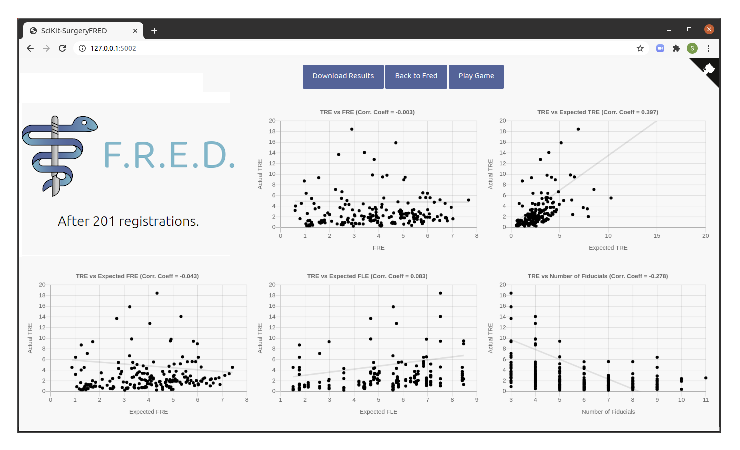
\includegraphics[width=0.9\linewidth]{images/systematic_error.eps}
			\caption{\label{fig:sys_error}Results of over 200 registrations with systematic error.}
	\end{center}
\end{figure}

It is noticeable that average \gls{TRE}s are higher than in cases where there is no
systematic error, while \gls{FRE} remains similar. This is as expected as \gls{FRE} will 
not account for systematic errors. This is a useful demonstration of this effect, though 
it might be more instructive to implement systematic errors in the game based method, see
Section \ref{sec:game_method}, to investigate the likely clinical impact of these
systematic errors.

\subsection{Statistical Significance}
As discussed in Section \ref{sec:methods} it is useful to perform tests of 
statistical significance on \fred{s} registration results. 
We used the function \href{https://docs.scipy.org/doc/scipy/reference/generated/scipy.stats.linregress.html}{stats.linregress} from {SciPy}\cite{2020SciPy-NMeth} to
perform a Wald Test against the null hypothesis that the slope is zero. For the
results shown in Figures \ref{fig:correlation}, \ref{fig:anis_error}, 
and \ref{fig:sys_error} there was no significant
relationship between actual \gls{TRE} and either actual or expected \gls{FRE}. There was
a significant relationship between actual \gls{TRE} and the expected \gls{TRE}. All
of these results are as expected.

Tests against the expected value of \gls{FLE} and the number of fiducial markers are
more problematic, as they are not continuous variables, which should be apparent 
when looking at the results charts. The reason for this is obvious for the number
of fiducial markers. The expected value of \gls{FLE} is clustered into groups as this
is only set once for a given target, however the registration for this target 
will be repeated each time a new fiducial marker is added beyond the minimum of 3. Hence 
if the user adds a total of 10 fiducial markers, this will create 8 registration 
results all with different \gls{TRE} and \gls{FRE}, but with a single value of 
expected \gls{FLE}.


\subsection{\fred for Research}
The results of the game based usability study described in Section \ref{sec:game_method}
are shown in 
Figure \ref{fig:usability}. As expected scores are 
highest when the actual \gls{TRE} is known. Interestingly it appears that when told only the expected value of the \gls{FLE} the students
tended to under treat the target more, resulting in lower overall scores. 


\begin{figure}
        \begin{center}
        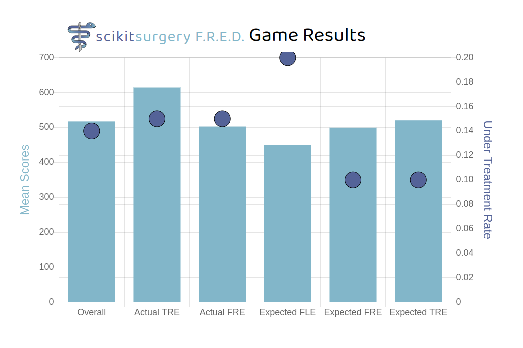
\includegraphics[width=0.5\linewidth]{usability.eps}
                \caption{\label{fig:usability}Average scores and treatment failure rates for the game based usability study.}
	\end{center}
\end{figure}

The statistical significance of the results was tested using a two sided T-test implemented
in {SciPy}'s\cite{2020SciPy-NMeth} \href{https://docs.scipy.org/doc/scipy/reference/generated/scipy.stats.ttest_ind.html}{stats.ttest{\textunderscore}ind} function.
Using a p-value of 0.05 none of the results were statistically significant. 
Currently there are only 100 data points (20 for each category), so this is not 
surprising. 



\section{Discussion}
SciKit-SurgeryFRED has proven useful for the teaching of fiducial based registration.
The results of the usability study 
are also of interest, however more participants are needed before any firm conclusions
can be drawn.
If we assume that additional data follow the same pattern as observed to date we
would need to run the game on a further 15 subjects to show statistical significance
on the difference in scores when using actual \gls{TRE}. In the case of the
\gls{FLE} we would need a further 30 participants. Given the ease with
which \fred can be deployed and used we hope to achieve this in the near future.

Currently \fred implements numerical measures for registration errors, however
in practice it may be better to use
graphical representations of registration error. An example is the use of
outline rendering to show the misalignment of anatomical edges during key hole 
surgery\cite{PMID:29663273}. Azimi et al. \cite{10.1007/978-3-030-59716-0_7} 
provide a similar example of a neuro-surgical guidance system where the 
registration error is communicated to the surgeon via misalignment of 
external anatomy. Such a method could be relatively easily implemented in \fred, with
gamification used to measure its effectiveness. 

Currently \fred is limited to rigid registration using point correspondence, however, 
there is no architectural reason why it could not be used to examine the 
effects of registration uncertainty more generally. It may be useful to implement 
more general error prediction models for rigid registrations\cite{4359072,5629373}.

Surface based registration has long been proposed as a way to improve 
registration accuracy for neurosurgery \cite{736031} and is 
is now integrated into commercial systems with mixed results \cite{mongen2020}.
\fred could in 
theory be extended include different registration methods, though obviously would 
require a more inclusive name. As we move to non rigid and 
probabilistic registrations, the correct interpretation of registration 
uncertainty will become more challenging \cite{10.1007/978-3-030-59716-0_26}.

\section{Conclusion}
Understanding registration uncertainty is essential for the correct 
use of image guided surgery. However there is a lack of tools to 
aid teaching and research.
We have presented \fred and demonstrated its use for teaching and research. 
\fred{s} ease of use enables it be deployed and demonstrated rapidly. However as
it is entirely open source and readily available \fred can also be applied to 
specific user's research questions. 




%Weaknesses:
%Useability study needs more samples, plus it should include a Null case (no information.

%Future work;
%We will include the FLE in the game log file, so we can examine what happens to performance under different conditions of FLE.

%Use FRED to examine other registration methods, for example a skin surface based method as used by medtronic.

%Use FRED to examine other ways of communicating registration error, for example raphical methods like (several, but include Thompson 2018)

\section{Open Access and Open Data}
This research was funded in whole, or in part, by the Wellcome Trust [203145Z/16/Z]. 
For the purpose of Open Access, the author has applied a CC BY public copyright licence to any Author Accepted Manuscript version arising from this submission.
The registration data described in Sections \ref{sec:methods} and \ref{sec:results} can be downloaded from \href{https://doi.org/10.5281/zenodo.4434278}{https://doi.org/10.5281/zenodo.4434278}.


\section{Acknowledgements}
This work is supported by the Wellcome/EPSRC Centre for Interventional and Surgical Sciences (WEISS) [203145Z/16/Z]. Our thanks to Simone Foti for designing the SciKit-Surgery logo, and to Dr Mary Thompson for proof reading the manuscript.



%\bibliographystyle{spie2008/myspiebib}
\bibliographystyle{spmpsci}

\bibliography{surgeryfred-paper.bib}

\end{document}
